%======================================================================
\chapter{Introduction}
%======================================================================
This chapter gives motivation, history of related work, and how our results fit into the current body of knowledge.

%----------------------------------------------------------------------
\section{Motivation and Related Work}\label{sec:related-work}

\paragraph{}
These days online dating applications are all the rage for eligible singles, but before these apps made finding a date as easy as a swipe of the finger, one way people met potential suitors was through their social circle. Imagine you really like playing cupid and you happen to know $n$ heterosexual male and heterosexual female friends who are all single and looking for dates. Since you're such a good friend you know each of your friends' preferences over who they would like to be paired with in the opposite gender, and even who they deem unacceptable. You would like to set up your single friends together in $n$ pairs and you have a goal: you don't want your friends to mutually circumvent your dating suggestions. Say some are your friends are Adam, Bob, Amy, and Brianne. If you pair Adam and Amy together, and Bob and Brianne, but Adam and Brianne mutually prefer each other to Amy and Bob respectively then they might want to ditch their suggested dates for each other. You hope to avoid this.

\begin{figure}
\centering
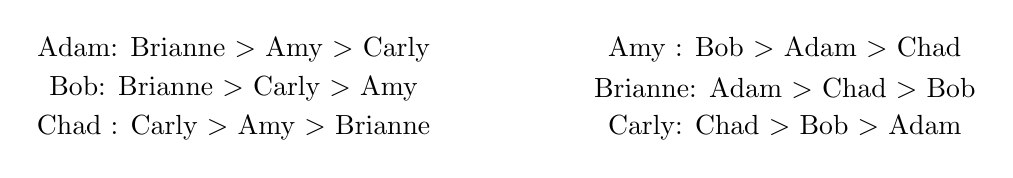
\begin{tikzpicture}

\draw (-2,2) node {Adam: Brianne $>$ Amy $>$ Carly};
\draw (-2,1.5) node {Bob: Brianne $>$ Carly $>$ Amy};
\draw (-2, 1) node {Chad : Carly $>$ Amy $>$ Brianne};
\draw (5, 2) node {Amy : Bob $>$ Adam $>$ Chad};
\draw (5, 1.5) node {Brianne: Adam $>$ Chad $>$ Bob};
\draw (5, 1) node {Carly: Chad $>$ Bob $>$ Adam};

\Vertex[x=0,y=0,L=$A$]{a1}
\Vertex[x=0,y=-1,L=$B$]{b1}
\Vertex[x=0,y=-2,L=$C$]{c1}

\Vertex[x=4,y=0,L=$A$]{a2}
\Vertex[x=4,y=-1,L=$B$]{b2}
\Vertex[x=4,y=-2,L=$C$]{c2}

\Edge[](a1)(a2)
\Edge[](b1)(b2)
\Edge[](c1)(c2)

\tikzstyle{EdgeStyle}=[dashed]
\Edge[](a1)(b2)
\end{tikzpicture}
\caption{A simple example of stable marriage}
\small
\begin{flushleft}
Solid edges indicate a matching and dashed edge indicates a blocking pair who prefer each other to their math. The pair $(\text{Chad},\text{Carly})$ will appear in any stable matching since they are each other's top choice.
\end{flushleft}
\end{figure}

\paragraph{}
In the previous dating game your single friends with their preferences form what is called by economists a two-sided matching market \cite{roth1992two}. The hope that your friends don't mutually want to ditch their dates is the condition of stability which is a highly desirable property in matching markets. A pair of friends who mutually prefer each other to their matches are called a blocking pair, and the existence of a blocking pair prevents stability. Other (perhaps more practical) examples of two-sided matching markets are the matching of medical school residents with hospitals for internships \cite{roth1996nrmp}, college applicants with colleges \cite{gale1962college}, and labour markets between employers and employees \cite{roth1992two}. The critical features of two-sided matching markets are the presence of two distinct groups without crossover who have interests in forming some mutual relationship with a member of the opposite group, and not only that but each member has preferences who they become involved with in the opposite group.
\paragraph{}
The abstract mathematical model of these phenomena is called a stable matching problem. In particular the model with two sides and strict preferences, referred to as Stable Marriage was first introduced by Gale and Shapley to investigate college admissions \cite{gale1962college}. Formally stable marriage asks for a matching in a bipartite graph such that no two vertices not matched together mutually prefer each other to their partners in the matching. See section \ref{sec:SM} of chapter $2$ for more detail. 

\paragraph{}
In Gale and Shapley's work they prove that stable matchings always exist for stable marriage problems through giving their famous deferred acceptance algorithm to compute stable matchings. See subsection \ref{SM:ALG} for details. For this work Shapley earned the Nobel Prize in Economics \cite{economic2012stable}. 

\paragraph{}
Stable matchings in two-sided markets come with a lot of interesting structure. In Gale and Shapley's original paper \cite{gale1962college} they observed that their algorithm favoured one side of the market over the other. Deferred acceptance has one side of the market play the role of proposers, and the other side playing the role of proposees. Proposers propose to proposees in order from their first to last choice and proposees tentatively accept or reject. They accept if they have no partner or they prefer the proposer to their current tentative partner. For a formal description see \ref{SM:ALG}. As it turns out the algorithm gives the proposers the best possible partner they could hope for in any stable matching. 
 
\paragraph{}
A major landmark in stable marriage was the work of Knuth \cite{knuthmariages}. Knuth demonstrated that when given two stable matchings, if all members of one side of the market like the first stable matching at least as well as the second then all members of the other side of the market like the second stable matching at least as well as the first. In plainer language the interests of both sides of the market are opposed.

\begin{figure}[h]
\centering
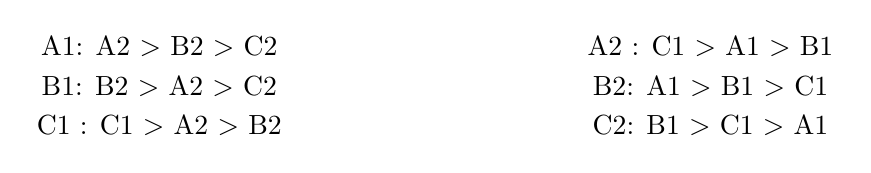
\begin{tikzpicture}
\draw (-2,2) node {A1: A2 $>$ B2 $>$ C2};
\draw (-2,1.5) node {B1: B2 $>$ A2 $>$ C2};
\draw (-2, 1) node {C1 : C1 $>$ A2 $>$ B2};
\draw (5, 2) node {A2 : C1 $>$ A1 $>$ B1};
\draw (5, 1.5) node {B2: A1 $>$ B1 $>$ C1};
\draw (5, 1) node {C2: B1 $>$ C1 $>$ A1};

\Vertex[x=0,y=0,L=$A$]{a1}
\Vertex[x=0,y=-1,L=$B$]{b1}
\Vertex[x=0,y=-2,L=$C$]{c1}

\Vertex[x=4,y=0,L=$A$]{a2}
\Vertex[x=4,y=-1,L=$B$]{b2}
\Vertex[x=4,y=-2,L=$C$]{c2}

\Edge[](a1)(a2)
\Edge[](b1)(b2)
\Edge[](c1)(c2)

\tikzstyle{EdgeStyle}=[dashed]
\Edge[](a1)(b2)
\Edge[](b1)(c2)
\Edge[](c1)(a2)
\end{tikzpicture}
\caption{Comparing two stable matchings}
\small
\begin{flushleft}
Solid edges indicate one stable matching and dashed edges indicate another stable matching. The solid matching is preferred by everyone on side $1$ and the dashed matching is preferred by everyone on side $2$.
\end{flushleft}
\end{figure}

\paragraph{}
In his work Knuth also mentions that the set of stable matchings of a two-sided market forms an algebraic structure called a distributive lattice. He credits Conway with the result. For details of a proof of this result see subsection \ref{SM:STRUCTURE} of chapter $2$ and in particular the proof of theorem \ref{theorem:lattice}.

\paragraph{}
One line of investigation related to our work in Chapter $3$ is to consider involves problems wherein each possible pairing in a stable matching problem is weighted by some possible utility, and our goal is to find a stable matching of maximum total weight. More formally if we let $E$ be the set of possible pairs in a stable matching instance we have a weight function $w : E \rightarrow \Q$ and our goal is to find a stable matching $M \subseteq E$ such that $\sum_{e\in M} w(e)$ is maximized over the set of all stable matchings. In a paper of Irving, Leather, and Gusfield \cite{irving1987efficient} they give an algorithm which solves weighted stable marriage by applying network flow theory methods to the set of ``rotations" in a problem instance. Another approach to solving weighted stable marriage would be via linear programming. Vande Vate was the first to formulate stable matchings in the stable marriage problem as the feasible region of a linear program and prove that the extreme points of his formulation were integer-valued vectors \cite{vate1989linear}. In doing so he implies a means of solving the weighted stable matching variant through the use of linear programming techniques. Vande Vate's formulation was only for the case of no unacceptable matches and his proof was complicated. Rothblum gave a formulation for the more general case where unacceptable matches were allowed, and Rothblum's proof via an extreme point argument was simpler than Vande Vate's original proof. \cite{rothblum1992characterization}.

\paragraph{}
Another line of investigation gaining more attention in recent years is the question of stable matching markets with more than two sides. In Knuth's work on stable matching he proposes a variant where we consider three-sided markets instead of two. In this context matchings are triples with one member from each side of the market, and matchings are stable if there does not exist a triple where each member mutually prefers the triple to the triple they are matched in. One important application for this type of model would be three-way kidney exchange in the context of organ transplant procedures in hospitals \cite{saidman2006increasing}. There are essentially two variants to this problem. The first is where each participant has preferences over the possible pairs they could be matched with.  Ng and Hirschberg \cite{ng1991three} consider this variant in their work and demonstrate that finding stable matchings for such problems in $NP$-hard.
\paragraph{}
The other possible variant, which we will focus our attention on in Chapter $4$, is the cyclic three-sided matching problem. In this problem participants from the first side of the market has preferences over the members of the second side (with indifference towards the third), the second side has preferences over the third, and the third side has preferences over the first side. It is an open conjecture by Knuth that stable matchings always exist for this problem when there are no unacceptable triples. As late as 2006 Eriksson et al. \cite{eriksson2006three} showed that for complete preference lists with at most 4 agents in each side there always exists a stable matching. In 2010 Biro et al. \cite{biro2010three} show a counterexample with 6 agents in each side but with incomplete preferences allowed. Later Farczadi et al. \cite{farczadi2014stable} proved that a natural approach through extending Gale and Shapley's deferred acceptance may be intractable by proving that the problem of deciding if any matching of two sides of a three-sided market can be extended to a stable three-sided matching is $NP$-complete.

\section{Surrounding Literature}

\paragraph{}
Gale and Shapley's work on stable marriage spawned a field of inquiry that brings together mathematicians, computer scientists, and economists in studying stable matching problems and their variants. We will discuss many of their results in this section. To learn more about the body of literature surrounding stable matching see the excellent texts of Roth and Sotomayor \cite{roth1992two}, Gusfield and Irving \cite{gusfield1989stable}, and Manlove \cite{manlove2013algorithmics}.

\paragraph{}
Once Gale and Shapley demonstrated that stable matchings always exist the next natural questions involved what the set of stable matchings in stable marriage problems look like. McVitie and Wilson \cite{mcvitie1971stable} gave an algorithm which found not just one stable matching, but the entire set of possible stable matchings for a given market. They also observed that in a stable matching where one side of the market are all matched with their best possible partner, like in deferred acceptance, the other side of the market are all matched with their worst possible partner. Another interesting structural result came from Gale and Sotomayor \cite{gale1985some} when they demonstrated that if someone was matched in any stable matching they were matched in all stable matchings. An immediate corollary of this is that all stable matchings of a given market have the same size.

\paragraph{}
Following Conway's Lattice Theorem \ref{theorem:lattice}, Blair  \cite{blair1984every} demonstrates the amazing fact that any finite distributive lattice is isomorphic to the set of stable matchings of some stable marriage problem. In Blair's paper he gives a construction which takes a finite distributive lattice and constructs a stable marriage problem whose set of stable matchings is isomorphic to the given lattice. Blair notes that his construction is not the most efficient possible in terms of the number of vertices in the stable marriage graph. In particular his construction has potentially exponential growth in the number of vertices in the stable marriage instance in terms of the number of elements of the lattice. Later Gusfield et al. \cite{gusfield1987every} show a more efficient construction which reduces the exponential growth to at worst polynomial growth.

\paragraph{}
One natural question which arises when first hearing about stable matching is: what happens when we remove sides from the market? That is, what happens when we allow all participants in the market to match with any other participant? Formally in stable marriage we were considering a constrained matching problem in bipartite graphs, but now we intend to lift the restriction that the graph is bipartite. This problem has been given the evocative name Stable Roommates. In Gale and Shapley's original work \cite{gale1962college} they consider this problem and give an example which shows the existence of a problem instance where no stable matching is possible.  Abeledo and Isaak \cite{abeledo1991characterization} advance this further by proving that a matching market is two-sided if and only if every reordering of the participants' preferences results in a market that has a stable matching.
\paragraph{}
In the stable roommates problem we would like an algorithm like the deferred acceptance procedure of Gale and Shapley that provides stable matchings, but since not every problem instance has a stable matching the algorithm should also be able to decide when a stable matching does not exist. In 1985, Irving \cite{irving1985efficient} provided such an algorithm. In collaboration with Gusfield \cite{irving1987efficient}, Irving showed as a consequence of his algorithm that for any stable roommates instance if a participant is matched in a stable matching they are matched in all stable matchings. As a corollary this implies that stable matchings in a given market all have the same size. While Irving has an algorithm to find a stable matching or report that none exist we need consider the question what sort of matching is desirable when no stable matching exists. A possible relaxation would be to ask for a matching with the least number of blocking pairs. It has been shown that it is $NP$-hard to find such a matching \cite{abraham2005almost}. For those without a complexity background, an optimization problem being $NP$-hard is considered strong evidence that no efficient algorithm exists for that problem. By efficient we mean that worst case running time is bounded above by a polynomial function of the size of the input specified in some reasonable encoding, for instance binary. See chapters $3$ and $4$ of Introduction to Algorithms \cite{cormen2009introduction} for an introduction to time complexity analysis and chapter $34$ for a discussion of $NP$-hardness.
\paragraph{}
Another natural question is to ask about what happens if indifference is allowed in stable marriage problems. By this we mean that we allow ties in participants' preferences. Once we allow ties we need to delineate between three different notions of stability. In any notion of stability a matching is considered stable if a blocking pair does not exist. A blocking pair with respect to a matching is a pair of vertices $u$ and $v$ that are not matched in the matching and that mutually prefer each other to their respective partners. In our original definition of stability in stable marriage both $u$ and $v$ strictly prefer each other to their matched partners. When ties are involved this notion of stability will be called weak-stability. Strong-stability says $u$ must strictly prefer $v$ to their partner but $v$ may strictly prefer, or be indifferent to, $u$ compared to their matched partner. Super-stability allows both $u$ and $v$ to either strictly prefer, or be indifferent to, each other compared to their matched partner.

\paragraph{}
Irving found that for stable marriage with ties, and where all possible pairings from both sides of market are acceptable to the participants, there always exists a weakly-stable matching \cite{irving1994stable}. It is also known that strong-stable and super-stable matchings need not always exist, but that polynomial time algorithms for deciding if they do and finding one if so exist. Irving resolves the super-stable case, while Kavitha et al. \cite{kavitha2004strongly} resolved the strongly-stable case. The work of Kavitha also covers the possibility of unacceptable matches, while an algorithm for finding strongly-stable matchings with unacceptable partners was given by Manlove \cite{manlove1999stable}. For weakly-stable matchings with unacceptable matches Manlove et al. \cite{manlove2002hard} demonstrated that weakly-stable matchings always exist, but they may have different sizes, which for previously mentioned variants was not the case. They showed that the problem of finding a largest weakly-stable matching is $NP$-hard.

\paragraph{}
We mentioned in the previous section (\ref{sec:related-work}) that the problem of finding a stable matching of optimal weight in a stable marriage problem is solvable in polynomial time. While this is true, the weighted stable roommates problem is considerably harder. Feder has shown that the problem of solving weighted stable roommates is $NP$-hard \cite{feder1992new}. Interestingly though the linear programming formulation Rothblum gave for weighted stable marriage can be used to find $\frac{1}{2}$-integral weighted stable roommates solutions. In 1994 he proved this result with Abeledo \cite{abeledo1994stable}. By $\frac{1}{2}$-integral we mean extreme point solutions of Rothblum's formulation take variable values in the set $\{0,\frac{1}{2},1\}$. While not solving the problem entirely, if the reader has an eye for applications we could imagine that a $\frac{1}{2}$ matching can have reasonable interpretations. For example splitting time in half between two contracts, or having a $50$ percent chance of being matched with a $\frac{1}{2}$ matched partner.

\section{Our Contributions and Outline}

\paragraph{}
Our first significant contribution to this body of theory is a simpler view of the linear programming formulation of weighted stable matching studied by Vande Vate and Rothblum. We present a short proof that Rothblum's formulation has integer-valued vectors for extreme points which uses only some elementary theory of polytopes and basic structural results on stable matchings. Our proof is inspired by the common paradigm of iterative rounding \cite{lau2011iterative}, yet takes a slightly different direction as one will see in Chapter $3$. We are hopeful that our proof technique can be used in the investigation of linear programming formulations for other stable matching type problems in the future since its simplicity leaves it wide open for extension.
\paragraph{}
Our other contributions are in the study of cyclic complete three-sided stable matchings as proposed by Knuth. We began our study in hopes of applying modern computing power to push higher the best known size for which it was known there is always a stable matching. As we previously mentioned it currently stands at $4$ and that result belongs to Eriksson and his collaborators. We propose a computer search framework for testing all instances of the problem for a given size. The framework is interesting because it allows for the cutting off of many instances simultaneously by not needing to explore their full preferences. It does this through the use of lemmas which are sufficient for proving existence of stable matchings, and eliminating from consideration instances that are equivalent to previously checked instances. 
\paragraph{}
We provide some new lemmas which are sufficient for concluding that an instance of the three-sided problem has stable matchings. Many of these lemmas are about finding a particular partial matching and applying ``induction" to get a stable matching in a smaller instance. Other lemmas try to satisfy all agents of a given side in a way that they are unwilling to prevent the matching from being stable. In the study of symmetry, we provide a definition of when two instances of the three-sided problem are symmetric and study the structure of equivalence classes under this symmetry.
\paragraph{}
In the next chapter we will give the reader the necessary background to understand our contributions, taking them through many of the the famous results previously mentioned along the way. They will also learn about linear programming and the methods of iterative rounding, and previous structural results in stable matching theory. The two chapters following preliminaries will detail our contributions to firstly polyhedral theory in stable matching, and secondly to three-sided stable matching problems. After that we conclude with a summary of what was studied, and provide many open avenues for the interested reader to begin exploring research problems in the theory of stable matchings based on our contributions in this thesis.
